\section{Mechanics of Continuous Media-Elasticity}
\subsection{Young's modulus}
The Young's modulus $E$ is also known as the elastic modulus.
It is used to predict how much a material extends under tension
or shortens under compression.

\begin{equation*}
  E = \frac{\sigma}{\epsilon} \qquad 
  [\si{\pascal} = \si{\newton\per\meter\squared}]
\end{equation*}

The experiment might be done using a rod as conceptually
illustrated in Figure~\ref{fig:stress_strain}.

\begin{figure}
  \begin{center}
    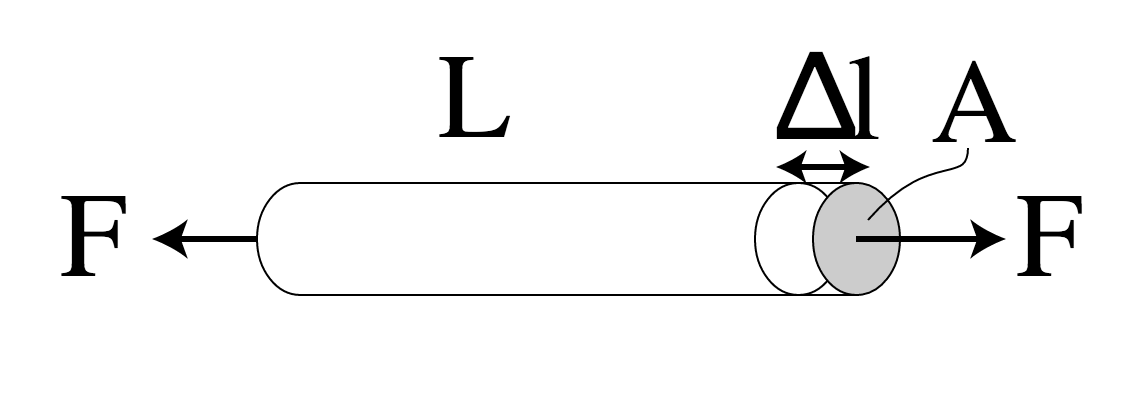
\includegraphics[scale=0.3]{stress_strain.png}
    \caption{Conceptual experiment to determine 
    Young's modulus $E = \sigma/\epsilon$
    from the stress $\sigma = F/A$ and strain $\epsilon = \Delta l/L$.}
    \label{fig:stress_strain}
  \end{center}
\end{figure}

We need a rod attached to the ceiling, a length-measuring tool
(eg: a Vernier scale) and some slotted masses of known mass.
First we measure the length $L$ of the rod
and its cross-sectional area $A$ when no mass is attached to it.
We then attach the different masses and measure for each one
the length of the rod and deduce the extension $\Delta L_i$.
From the weight of each mass $m_i$,
we compute the associated force $F_i = m_i \, g$.
We now have all needed information to plot
the stress-strain curve of the material.
We observe in Figure~\ref{fig:stress_strain_curve},
which shows the stress-strain curve of steel,
that the slope varies.
The tangent of the initial, linear portion of the curve
(during which is material is referred as elastic) 
is the Young's modulus.

\begin{figure}
  \begin{center}
    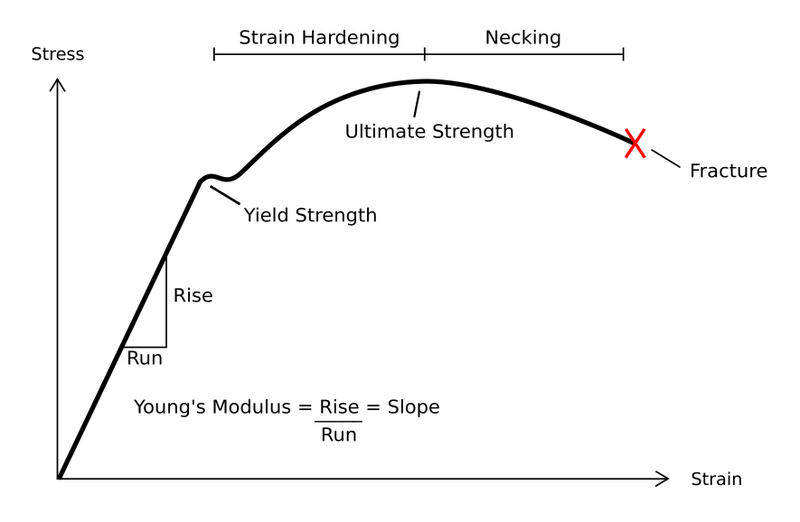
\includegraphics[scale=0.7]{stress_strain_curve.png}
    \caption{Stress-strain curve of steel.}
    \label{fig:stress_strain_curve}
  \end{center}
\end{figure}

Its order of magnitude is in $\si{\giga\pascal}$ for steel materials.

\subsubsection*{Stress and strain}
Note that \emph{stress} $\sigma$ is a physical quantity that 
expresses the internal forces that neighboring particles 
of a continuous material exert on each other,
while \emph{strain} $\epsilon$ is the measure of the deformation 
in terms of relative displacement of particles in the material.

\subsection{Poisson ratio}
The Poisson ratio $\nu$ is also known as
the coefficient of expansion on the tranverse axial.
It is the negative ratio of tranverse to axial strain.
If the material is stretched along the axial direction
\[
  \nu = -\frac{\dif\strain{trans}}{\dif\strain{axial}}
  = -\frac{\dif\strain{y}}{\dif\strain{x}}
  = -\frac{\dif\strain{z}}{\dif\strain{x}}
\]
Note that $\strain{axial}$ is defined positive for axial tension
(thus negative for compression).

An experiment to determine Poisson ratio can easily be done
using an iron rod and a system which measures the displacements
of the rod in the 3 directions.
We extend the rod following one direction,
then measure the axial strain and the tranverse one.

\begin{figure}
  \begin{center}
    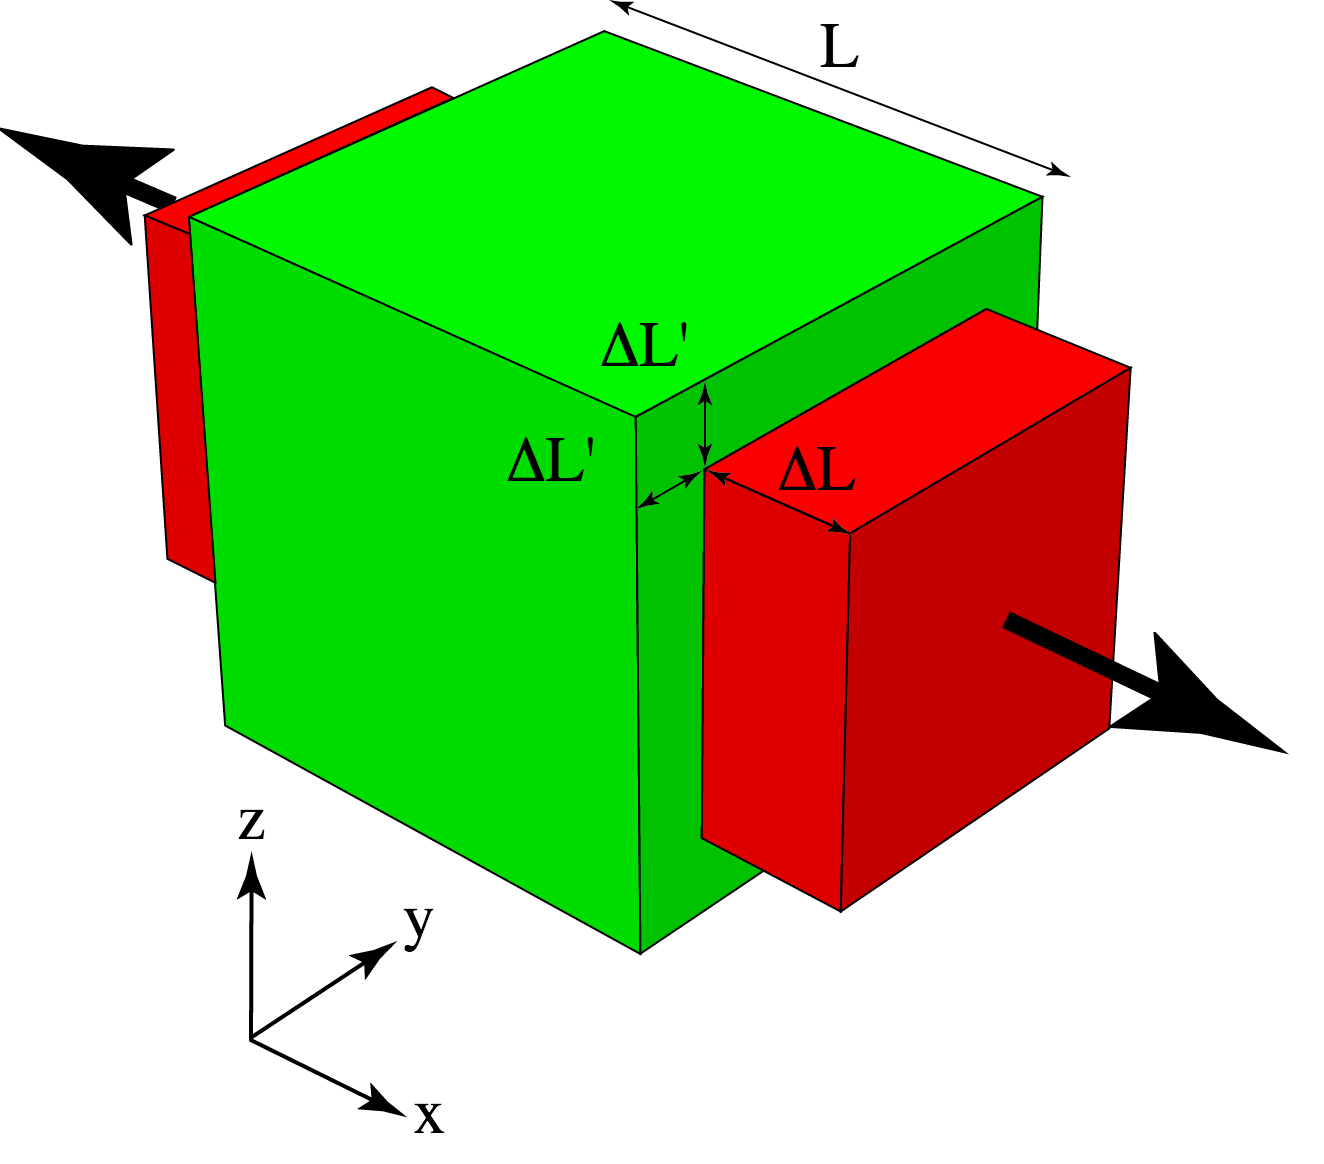
\includegraphics[scale=0.3]{poisson_ratio_scheme.png}
    \caption{Conceptual experiment to determine the Poisson ratio,
    defined in this picture as $\mu = - |\Delta L'/\Delta L|$.}
    \label{fig:poisson_ration_scheme}
  \end{center}
\end{figure}

The Poisson Ratio is dimensionless, it has no units.
Its value for most materials varies between $-1.0$ and $0.5$
and has an average value of $0.3$.

\subsection{Strain tensor}
The components of the strain matrix ${\bf \strain{}}$
are obtained using this relation
\[ 
  \strain{ij} = \frac{1}{2} \left(\frac{\partial u_i}{\partial u_j}
  + \frac{\partial u_j}{\partial u_i}\right)
\]
where $u=(u_x,u_y,u_z)$ is the displacement vector.

We derive that, following notation of Figure~[TO ADD],
\begin{align*}
  \strain{1} &= \strain{x}\cos^2{\theta_1} + \strain{y}\sin^2{\theta_1}
  + 2 \strain{xy}\sin{\theta_1}\cos{\theta_1} \\
  \strain{2} &= \strain{x}\cos^2{\theta_2} + \strain{y}\sin^2{\theta_2}
  + 2 \strain{xy}\sin{\theta_2}\cos{\theta_2} \\
  \strain{3} &= \strain{x}\cos^2{\theta_3} + \strain{y}\sin^2{\theta_3}
  + 2 \strain{xy}\sin{\theta_3}\cos{\theta_3}
\end{align*}

\subsection{Stress on a rigid body}
If we have 
\[ \sigma_{zz} = \rho g (z-H) + p \]
the associated body forces and surface forces on each face are
\begin{enumerate}
  \item at $z=0$
  \[ \sigma_{zz}^{z=0} = \frac{F_{z=0}}{L^2} \]
  which gives
  \[ F_{z=0} = - V \rho g + p L^2 \]
  We identify two component, the first $-V \rho g$ is the body force
  (corresponding to its weight) and the second $p$ is the surface force.
  \item at $z=H$
  \[ F_{z=H} = p L^2 \]
  which is only the surface force.
\end{enumerate}

Note that the forces on the other are all equal to $0$.
We conclude that $p$ is the traction's stress.

The force exerced by the body on its support is the opposite
of $F_{z=0}$.
